\section{Kubernetes}

In this section we will dive into the topic of Kubernetes. We start by shortly overviewing the Kubernetes architecure. Then we expand on the Kubernetes resources, their kinds and their role in the target application environment. Finally, we consider the security of Kubernetes.

\subsection{Overview}

Kubernetes, also known as K8s, is an open source system for automating deployment, scaling, and management of containerized applications. It groups containers that make up an application into logical units for easy management and discovery. Kubernetes builds upon 15 years of experience of running production workloads at Google, combined with best-of-breed ideas and practices from the community. \cite{kubernetes}.

IBM defines Kubernetes as an open source \textbf{container orchestration platform} for scheduling and automating the deployment, management and scaling of containerized applications. Today, Kubernetes and the broader ecosystem of container-related technologies have merged to form the building blocks of modern cloud infrastructure. This ecosystem enables organizations to deliver a highly productive hybrid multicloud computing environment to perform complex tasks surrounding infrastructure and operations. It also supports cloud-native development by enabling a build-once-and-deploy-anywhere approach to building applications. \cite{ibm-kubernetes}.

It is important to emphasize that the Kubernetes abstracts the actual machines (nodes) from the user. Nodes can be physical on-premises servers, or VMs that reside either on-premises or at a cloud provider. Kubernetes takes on the responsibilty of figuring out the deployment target for a particular application. That is, user only defines the desired state of the infrastructure using YAML or JSON configuration files. Kubernetes then creates all the workloads based on the applied configuration.

\subsection{Kubernetes Architecture}

While Kubernetes requires at least three nodes to run, there are some implementation designed for the local use, which emulate this concept (see Subsection~\ref{sec:other-kubernetes-implementations}). The master node is called control plane. The control plane manages the worker nodes and the Pods in the cluster. In production environments, the control plane usually runs across multiple computers and a cluster usually runs multiple nodes, providing fault-tolerance and high availability. Worker nodes host the actual workload inside the cluster. Figure~\ref{img:kubernetes-architecture} provides a simple high-level overview of a typical Kubernetes cluster with a Control Plane and three worker nodes.

\begin{figure}[!hbt]
	\begin{center}
		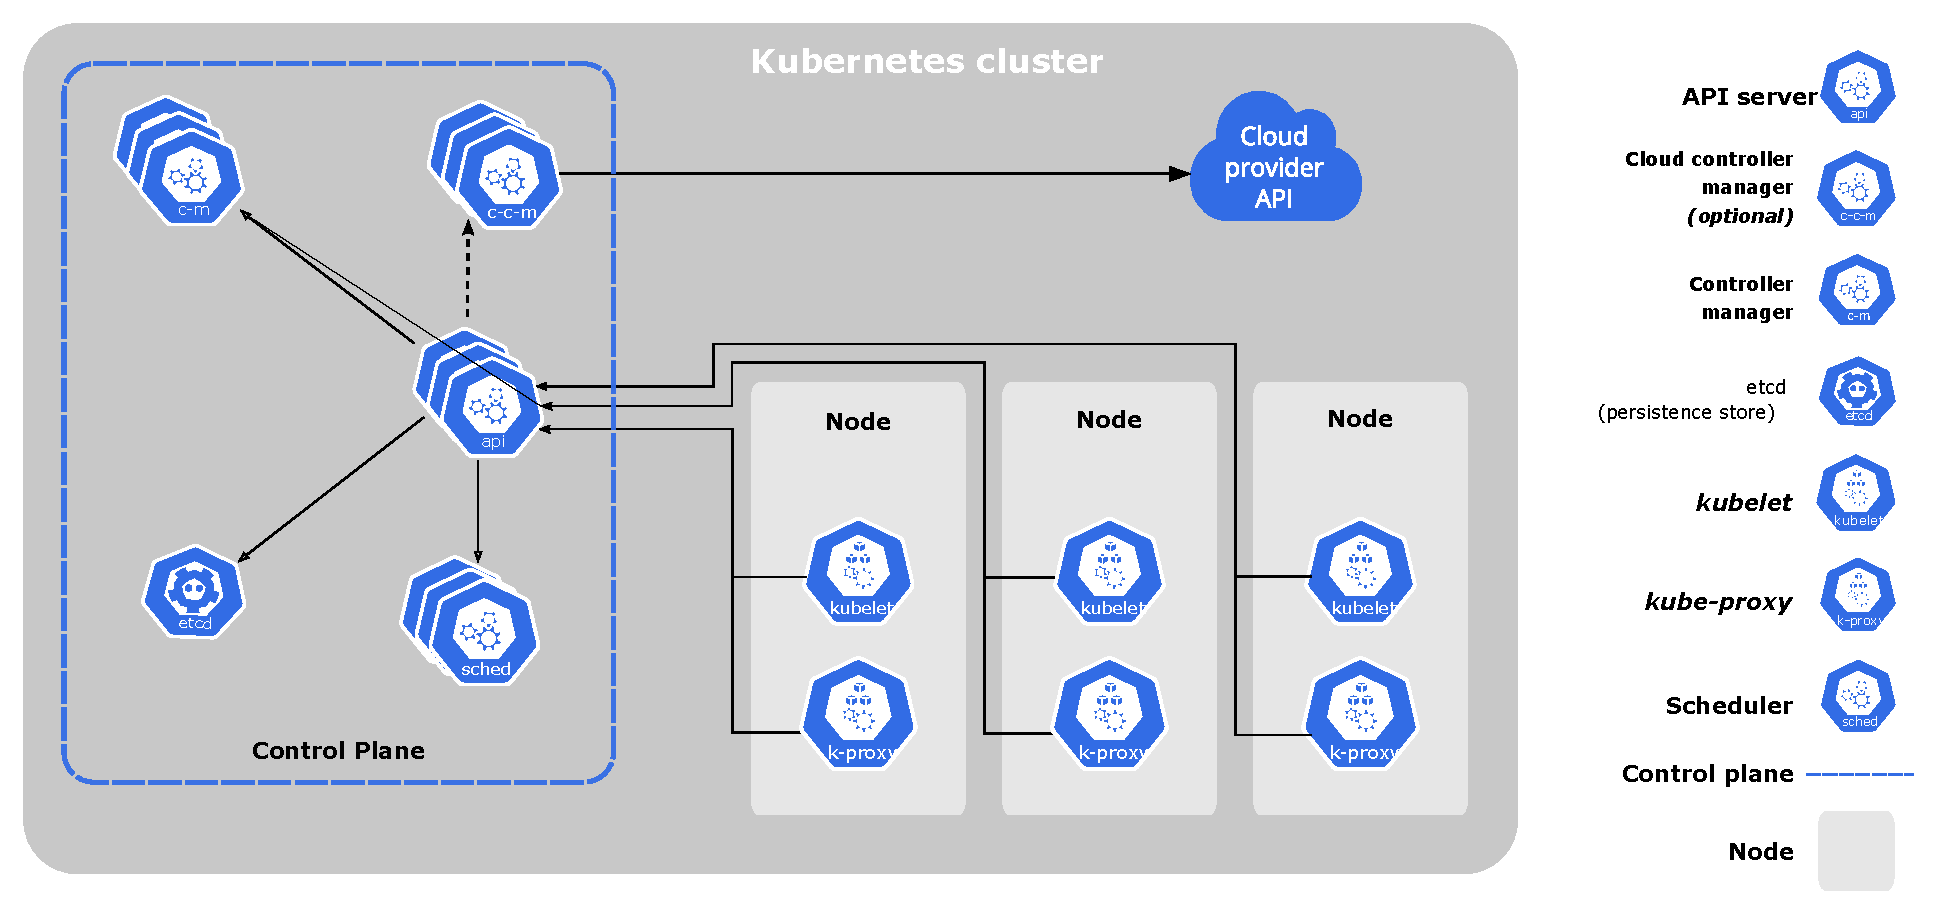
\includegraphics[width=0.85\textwidth]{images/components-of-kubernetes.pdf}
        \caption{Kubernetes cluster architecure overview with its main components.}
		\label{img:kubernetes-architecture}
	\end{center}
\end{figure}

\subsubsection*{Control Plane overview}

Control plane runs the following components: 
\begin{itemize}
\item \textbf{kube-apiserver} \\
Kube-apiserver exposes the Kubernetes API, which is acting as a frontend for the Kubernetes control plane.
\item \textbf{etcd} \\
Etcd is a key-value store, where all of the cluster data is stored.
\item \textbf{kube-scheduler} \\
Each time a new pod is created, it is passed to the kube-scheduler, which assigns the pod to the specific node to run on (based on individual and collective resource requirements, hardware/software/policy constraints, affinity and anti-affinity specifications, data locality, inter-workload interference, and deadlines).
\item \textbf{kube-controller-manager} \\
Each Kubernetes resource has its own controller (e.g. NodeController, JobController, ServiceAccountController); all of them are compiled as one binary called kube-controller-manager.
\item \textbf{cloud-controller-manager} \\
Cloud-controller-manager embeds cloud-specific control logic. It differs depending on the cloud provider or can be absent completely, when running Kubernetes locally.
\end{itemize}

\subsubsection*{Worker Node overview}

Each worker node has a kubelet and kube-proxy installed. Kubelet is an agent that manages runnning pods and containers. Kube-proxy is a network proxy that implements parts of the Kubernetes service concept. It maintains network rules on nodes, making in- outside-cluster communitcation possible.

Then, of course, each worker node has a set of running pods. A typical use would involve multiple running applications. Depending on the size of the node and the application resoucre consumption it can accomodate on average from one to a few dozens applications with various business purposes.

\subsection{Kubernetes Resources}

Kubernetes resources are fundamental components that define various entities within a Kubernetes cluster. Resources are objects that represent the desired state and configuration of the infrastructure, applications, and services running on the cluster. Kubernetes provides a range of resources that enable developers and operators to define, manage, and scale containerized applications, network policies, storage requirements, and more. These resources are defined declaratively in YAML or JSON files, which makes infrastructure setup consistent and reproducible.

Among key Kubernetes resoucres are:
\begin{itemize}
    \item \textbf{Pods} \\
        Pod is the atomic workload unit in the Kubernetes cluster. It encapsulates one or more containers that share the same network. It represents a single instance of a running application.
    \item \textbf{Deployments} \\
        Deployments are a higher level of abstraction for the Pods. They allow to define replica count and rollout/rollback strategy for the updates, which can be used to ensure availability for the application.
    \item \textbf{Services} \\
        Services provide a communication layer for the pods inside one cluster. Being an abstraction over the pods' network, they provide reliable access to the selected workloads, while serving as a Load Balancer. 
    \item \textbf{ConfigMaps} and \textbf{Secrets} \\
        ConfigMaps and Secrets allow users to store data outside the workload. ConfigMaps are usually used to store non-sensitive information like environment and application configuration parameters. Secrets are a more secure resource designed for API keys, passwords and other sensitive data.
    \item \textbf{PersistentVolumes} and \textbf{PersistentVolumeClaims} \\
        These resources enable stateful applications to request and mount durable storage within a cluster, allowing data to persist independently of the Pod lifecycle.
\end{itemize}

Above are the most commonly used resources, which we also leverage in the practical part of the paper. Therefore, it is important that the reader understands the position and the purpose of each resource in the cluster infrastructure.

\subsubsection*{Workloads}

Minimal computing units in Kubernetes are Containers, which are running in Pods. However, to simplify the management of Pods, Kubernetes has workload resources, which manage the set of Pods. They make sure the desired number of Pods of right kind are running to match the declaration.

Deployments and ReplicaSets are a good fit for stateless applications. Each pod in the Deployment is interchangebeable. Deployments are easily scalable and have built-in versioning and rollout mechanisms.

StatefulSet allows to create sets of stateful applications. They might share the same PersistentVolume and replicate data between each other.

DaemonSet defines Pods that provide node-local facilities. These might be fundamental to the operation of your cluster, such as a networking helper tool, or be part of an add-on.

Job and CronJob define tasks that run to completion and then stop. Jobs represent one-off tasks, whereas CronJobs recur according to a schedule.

\subsubsection*{Networking}

Kubernetes networking model makes Pods look like VMs in the networking aspect. Pods on any nodes can communicate with each other without NAT. Containers inside the same Pod share its network meaning that they can reach each other using localhost.

Kubernetes networking addresses four concerns:
\begin{itemize}
\item Containers within a Pod use networking to communicate via loopback.
\item Cluster networking provides communication between different Pods.
\item The Service API lets you expose an application running in Pods to be reachable from outside your cluster.
\item Ingress provides extra functionality specifically for exposing HTTP applications, websites and APIs.
\item You can also use Services to publish services only for consumption inside your cluster.
\end{itemize}

\subsubsection*{Storage}

Kubernetes does not ship a particular implementation of storage. However, it provides a range of resources that define the storage concept and supports different types of volumes. A Pod can use any number of volume types simultaneously. Ephemeral volume types have a lifetime of a pod, but persistent volumes exist beyond the lifetime of a pod. When a pod ceases to exist, Kubernetes destroys ephemeral volumes; however, Kubernetes does not destroy persistent volumes. For any kind of volume in a given pod, data is preserved across container restarts.

At its core, a volume is a directory, possibly with some data in it, which is accessible to the containers in a pod. How that directory comes to be, the medium that backs it, and the contents of it are determined by the particular volume type used.

PersistentVolumes and PersistentVolumeClaims are the resources kinds most important to understand here.
\begin{itemize}
\item A PersistentVolume (PV) is a piece of storage in the cluster that has been provisioned by an administrator or dynamically provisioned using Storage Classes. It is a resource in the cluster just like a node is a cluster resource. PVs are volume plugins like Volumes, but have a lifecycle independent of any individual Pod that uses the PV. This API object captures the details of the implementation of the storage, be that NFS, iSCSI, or a cloud-provider-specific storage system.
\item A PersistentVolumeClaim (PVC) is a request for storage by a user. It is similar to a Pod. Pods consume node resources and PVCs consume PV resources. Pods can request specific levels of resources (CPU and Memory). Claims can request specific size and access modes (e.g., they can be mounted ReadWriteOnce, ReadOnlyMany or ReadWriteMany). Once and Many here refer to a number of Pods that can perform the read or write simultaneously.
\end{itemize}

\subsection{Infrastructure Security}

When we are talking about the infrastructure security, we must consider multiple layers. Going from the top to the bottom, we start with the security measurements taken on the Cloud provider side. In most cases this is not something we can affect and the security of different Cloud providers varies significantly. Unfortunately, this is out of scope of this paper, but all of the "big five" Cloud providers (AWS, Azure, Google Cloud, Alibaba and IBM) maintain high security standarts and security risks generally should not be a concern for their end users. Then, we get to the cluster itself. On the cluster level we must consider the security of the nodes, security of the cluster components and their configuration. At this layer we have already some space for the misconfigurations to appear. Here we can evaluate the security of the single components using some of the security scanners presented in \nameref{sec:kubernetes-security-automation}. Lastly, we get to the application level, where the security of the application code, Kubernetes resoucre configuration, libraries, dependencies and base images is the main concern. Again, this is the layer, where the developers have the most access to, thus, providing a lot of space for the possibility of a human error. In this paper we mostly work on this level when we do our research.

Officially, The Linux Foundation provides only some security guidelines for each of the layers. However, bundled with Kubernetes we get a few means to keep the security under control. Below we present an overview of the Kubernetes security recommendations, RBAC and Data security inside Kubernetes.

\subsubsection*{Kubernetes security recommendations}

This section gathers the official security recommendations provided by the Kubernetes. They provide a list of concerns for each level of the cloud infrastructure. Cloud infrastructure can be viewed as a composition of four layers as displayed by the Figure~\ref{img:cloud-security}.

\begin{figure}[!hbt]
	\begin{center}
		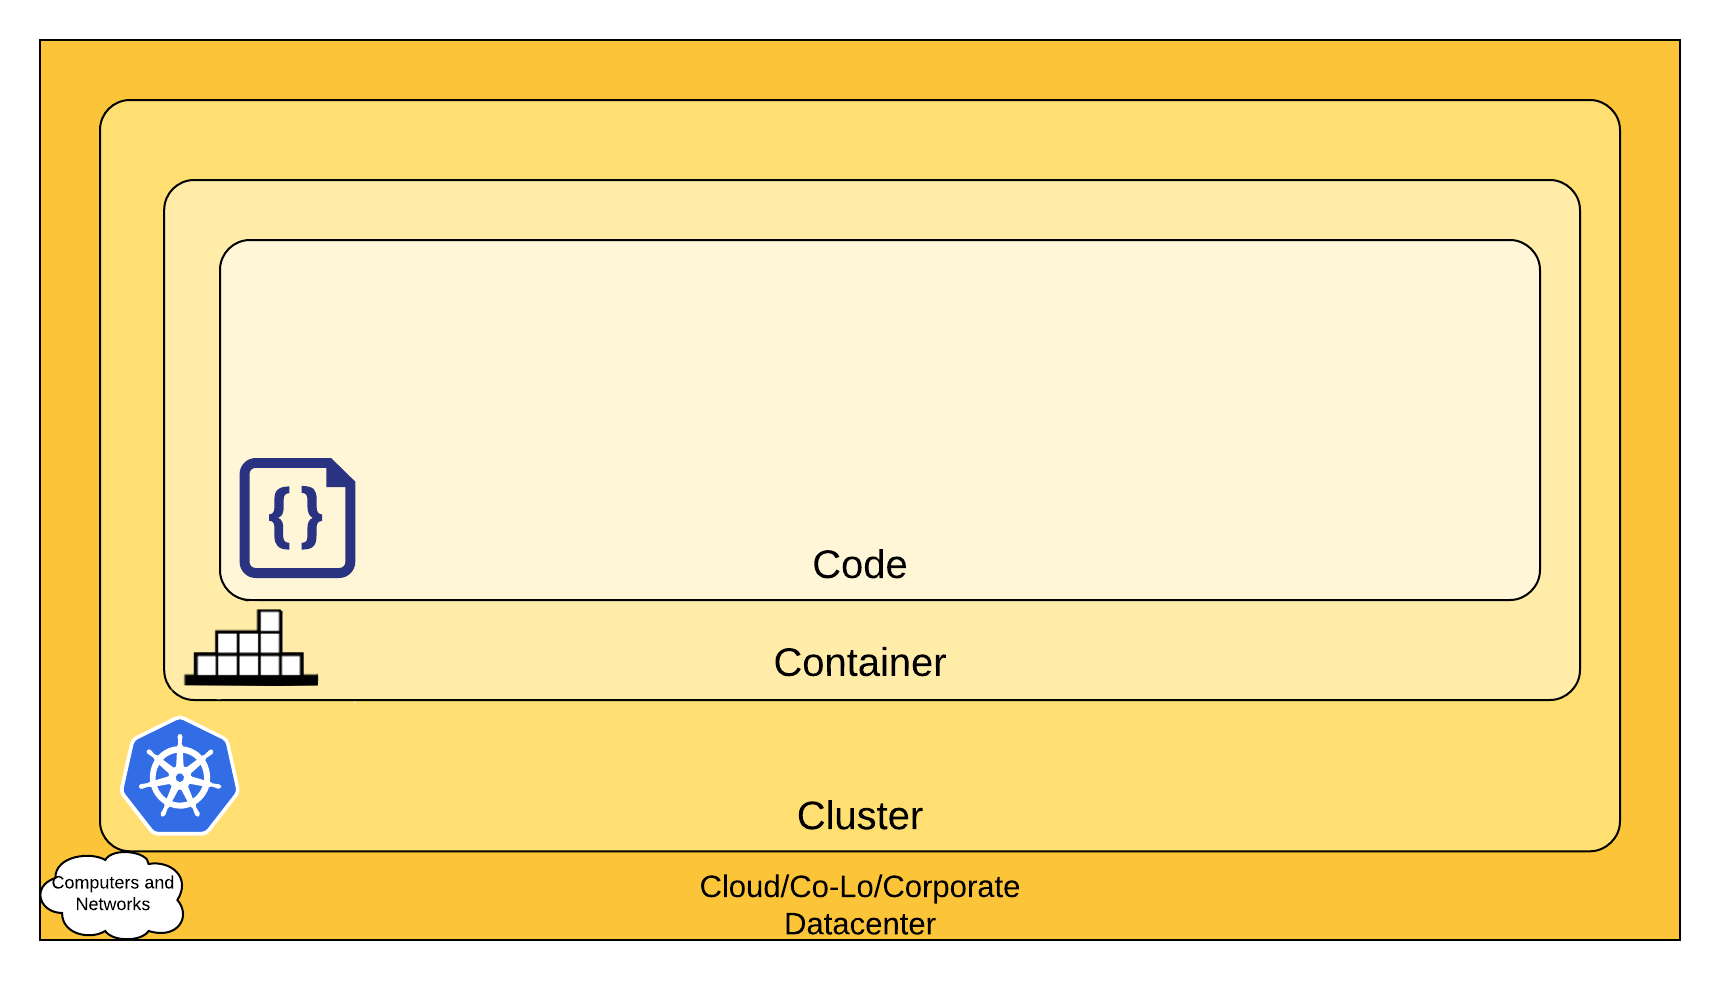
\includegraphics[width=0.75\textwidth]{images/cloud-security.png}
        \caption{Four layers of the cloud infrastructure.}
		\label{img:cloud-security}
	\end{center}
\end{figure}

Each layer is built upon the previous one and its security depends on the security of the outer layers. It is, therefore, important to maintain high security standarts on base levels (Cloud, Cluster, Container).

\begin{enumerate}

\item \textbf{Cloud} \\
Each cloud provider has its own security policies and guidelines. There are, however, some general infrastructure-level security best advice described by in the Table~\ref{tab:cloud-security-recommendations}.

\begin{table}[H]
    \begin{center}
        \begin{tabular}{ | p{.20\textwidth} | p{.80\textwidth} | } 
         \hline
         \textbf{Area of Concern for Kubernetes Infrastructure} & \textbf{Recommendation} \\ 
         \hline
         Network access to API Server (Control plane) & All access to the Kubernetes control plane is not allowed publicly on the internet and is controlled by network access control lists restricted to the set of IP addresses needed to administer the cluster. \\ 
         \hline
         Network access to Nodes (nodes)  & Nodes should be configured to only accept connections (via network access control lists) from the control plane on the specified ports, and accept connections for services in Kubernetes of type NodePort and LoadBalancer. If possible, these nodes should not be exposed on the public internet entirely. \\ 
         \hline
         Kubernetes access to Cloud Provider API & Each cloud provider needs to grant a different set of permissions to the Kubernetes control plane and nodes. It is best to provide the cluster with cloud provider access that follows the principle of least privilege for the resources it needs to administer. \\
         \hline
         Access to etcd & Access to etcd (the datastore of Kubernetes) should be limited to the control plane only. Depending on your configuration, you should attempt to use etcd over TLS. \\
         \hline
         etcd Encryption & Wherever possible it's a good practice to encrypt all storage at rest, and since etcd holds the state of the entire cluster (including Secrets) its disk should especially be encrypted at rest. \\
         \hline
        \end{tabular}
    \end{center}
    \caption{Security recommendations for the Cloud layer.}
    \label{tab:cloud-security-recommendations}
\end{table}

\item \textbf{Cluster} \\
There are two cluster security concerns that could be addressed: securing the configurable cluster components and securing the applications running in the cluster.

There are a few things to consider regarding the application security:
\begin{itemize}
\item RBAC Authorization (Access to the Kubernetes API)
\item Authentication	
\item Application secrets management (and encrypting them in etcd at rest)
\item Ensuring that pods meet defined Pod Security Standards
\item Quality of Service (and Cluster resource management)
\item Network Policies
\item TLS for Kubernetes Ingress
\end{itemize}

\item \textbf{Container} \\
Securing containers is a vast topic, which deserves its own chapter. There are, nevertheless, a few general recommendation provided by the Kubernetes, which you can find in the Table~\ref{tab:container-security-recommendations}.

\begin{table}[H]
    \begin{center}
        \begin{tabular}{ | p{.20\textwidth} | p{.80\textwidth} | } 
        \hline
        \textbf{Area of Concern for Containers} & \textbf{Recommendation} \\ 
        \hline
        Container Vulnerability Scanning and OS Dependency Security & As part of an image build step, you should scan your containers for known vulnerabilities. \\ 
        \hline
        Image Signing and Enforcement & Sign container images to maintain a system of trust for the content of your containers. \\ 
        \hline
        Disallow privileged users & When constructing containers, create users inside of the containers that have the least level of operating system privilege necessary in order to carry out the goal of the container. \\
        \hline
        \end{tabular}
    \end{center}
    \caption{Security recommendations for the Container layer.}
    \label{tab:container-security-recommendations}
\end{table}

\item \textbf{Code} \\
When it comes to code, the developers have the most flexibility to design secure applications. There are a lot of issues to address, which may vary significantly from application to application depending on its purpose, architecture and framework base. Kubernetes documentation gives a handful of recommendations regarding this topic, which are displayed below in the Table~\ref{tab:code-security-recommendations}.

\begin{table}[H]
    \begin{center}
        \begin{tabular}{ | p{.20\textwidth} | p{.80\textwidth} | } 
        \hline
        \textbf{Area of Concern for Code} & \textbf{Recommendation} \\ 
        \hline
        Access over TLS only & If your code needs to communicate by TCP, perform a TLS handshake with the client ahead of time. With the exception of a few cases, encrypt everything in transit. Going one step further, it's a good idea to encrypt network traffic between services. This can be done through a process known as mutual TLS authentication or mTLS which performs a two sided verification of communication between two certificate holding services. \\ 
        \hline
        Limiting port ranges of communication & This recommendation may be a bit self-explanatory, but wherever possible you should only expose the ports on your service that are absolutely essential for communication or metric gathering. \\ 
        \hline
        3rd Party Dependency Security & It is a good practice to regularly scan your application's third party libraries for known security vulnerabilities. Each programming language has a tool for performing this check automatically. \\
        \hline
        Static Code Analysis & Most languages provide a way for a snippet of code to be analyzed for any potentially unsafe coding practices. Whenever possible you should perform checks using automated tooling that can scan codebases for common security errors. \\
        \hline
        Dynamic probing attacks & There are a few automated tools that you can run against your service to try some of the well known service attacks. These include SQL injection, CSRF, and XSS. One of the most popular dynamic analysis tools is the OWASP Zed Attack proxy tool. \\
        \hline
        \end{tabular}
    \end{center}
    \caption{Security recommendations for the Code layer.}
    \label{tab:code-security-recommendations}
\end{table}
                      
\end{enumerate}

\subsubsection*{Role Based Access Control}

\subsubsection*{Data security}

\subsection{Other Kubernetes Implementations}
\label{sec:other-kubernetes-implementations}

\subsubsection*{Openshift}

\subsubsection*{Rancher Desktop}